\documentclass[12pt,a4paper]{article}
\usepackage{etex,datetime,setspace,latexsym,amssymb,amsmath,amsthm}
\usepackage{fancybox,dialogue,float,wrapfig,enumerate,microtype}
\usepackage{verbatim,xcolor,multicol,titlesec,tabularx,mdframed}
\newcommand{\alt}{\textrm{alt}}
\newcommand{\info}{\textrm{info}}
\usepackage[utf8]{inputenc}
\usepackage[pdftex]{hyperref}
\usepackage[bottom=3cm,footskip=15mm]{geometry}
% \parindent0cm
% \parskip1em

\usepackage{tikz}
\usetikzlibrary{arrows,trees,positioning,shapes,patterns}
\usetikzlibrary{intersections,calc,fpu,decorations.pathreplacing}

\tikzstyle{index on}=[inner sep=2pt, white, circle, fill=black]
\tikzstyle{index off}=[inner sep=2pt, black, circle, draw]
\tikzstyle{index gray}=[inner sep=2pt, black, circle, fill=lightgray]
\tikzstyle{opaque}=[fill=gray,fill opacity=.1]
\tikzstyle{counter}=[densely dashed]


%packages for theorems, definitions, etc.
\usepackage{amsthm}
\newtheorem{prop}{Proposition}
\newtheorem{lemma}{Lemma}
\newtheorem{defi}{Definition}

\usepackage[T1]{fontenc} % better fonts

% Haskell code listings in our own style
\usepackage{listings,color}
\definecolor{lightgrey}{gray}{0.35}
\definecolor{darkgrey}{gray}{0.20}
\definecolor{lightestyellow}{rgb}{1,1,0.92}
\definecolor{dkgreen}{rgb}{0,.2,0}
\definecolor{dkblue}{rgb}{0,0,.2}
\definecolor{dkyellow}{cmyk}{0,0,.7,.5}
\definecolor{lightgrey}{gray}{0.4}
\definecolor{gray}{gray}{0.50}
\lstset{
  language        = Haskell,
  basicstyle      = \scriptsize\ttfamily,
  keywordstyle    = \color{dkblue},     stringstyle     = \color{red},
  identifierstyle = \color{dkgreen},    commentstyle    = \color{gray},
  showspaces      = false,              showstringspaces= false,
  rulecolor       = \color{gray},       showtabs        = false,
  tabsize         = 8,                  breaklines      = true,
  xleftmargin     = 8pt,                xrightmargin    = 8pt,
  frame           = single,             stepnumber      = 1,
  aboveskip       = 2pt plus 1pt,
  belowskip       = 8pt plus 3pt
}
\lstnewenvironment{code}[0]{}{}
\lstnewenvironment{showCode}[0]{\lstset{numbers=none}}{} % only shown, not compiled

% will the real phi please stand up
\renewcommand{\phi}{\varphi}

% load hyperref as late as possible for compatibility
\usepackage[pdftex]{hyperref}
\hypersetup{pdfborder = {0 0 0}, breaklinks = true}


\title{A Model Checker for Inquisitive Semantics}
\author{Bo Flachs \& Wessel Kroon}
\date{\today}
\hypersetup{pdfauthor={Bo Flachs \& Wessel Kroon}, pdftitle={A Model Checker for Inquisitive Semantics}}

\begin{document}

\maketitle

\begin{abstract}
In this report we discuss a Haskell model checker for basic inquisitive semantics, called \textit{InqB}. Inquisitive semantics is designed to be able to analyse not only declarative natural language sentences, but also interrogatives. We give a short introduction into the technicalities of the framework, after which we discuss its implementation in Haskell step by step. We use QuickCheck to check several well-known facts about the framework \textit{InqB}.
\end{abstract}

\tableofcontents

\clearpage

\section{Introduction}\label{sec: Introduction}
Inquisitive semantics is a relatively new framework in which information exchange can be analysed. In addition to declarative sentences, questions can be analysed in this semantic framework. In this report we describe how we build a model checker for the most basic version of inquisitive semantics, \textsf{InqB}.

We have two goals in mind. Firstly, we want to be able to evaluate formulas relative to specified models. And secondly, we want to check several theorems using QuickCheck.

In Section 2 we will give a concise introduction to \textsf{InqB}, taking our cue from \cite{inquisitive19}. Section 3 concerns itself with the implementation of \textsf{InqB} and our model checker in Haskell. Thereafter, in Section 4, we give some examples. In Section 5 we perform some simple tests after which we give our conclusion in Section 6.



\section{Inquisitive Semantics}\label{sec: InqB}
% Language
Below we will give a brief overview of \textsf{InqB}, taking our cue from \cite{inquisitive19}.\footnote{Basic notions such as propositions, information states and alternatives are treated comprehensively in Chapter 2 of \cite{inquisitive19}, while the language, models and semantics of \textsf{InqB} are treated in Chapter 4 of the same book.}

Any standard first-order language $\mathcal{L}$, containing a set of function symbols $\mathcal{F}_\mathcal{L}$ and a set of relation symbols $\mathcal{R}_\mathcal{L}$, is also a language of \textsf{InqB}. In our model checker we do not concern ourselves with function symbols, therefore we will not mention them in the remainder of this report. As for the constants in a language, we will assume that for each individual in the domain of a model we will have a constant in our language. We define models of \textsf{InqB} below.

% Model
\begin{defi}\label{def: InqBModel}
An \textsf{InqB} model for a first-order language $\mathcal{L}$ is a triple $M=\langle W,D,I\rangle$, where:
\begin{itemize}
\setlength\itemsep{-0.3em}
    \item $W$ is a non-empty set of possible worlds;
    \item $D$ is a non-empty set of individuals;
    \item $I$ is a map that associates every $w\in W$ with a first order structure $I_w$ such that:
    \begin{itemize}
    \setlength\itemsep{-0.3em}
        \item for every $w\in W$, the domain of $I_w$ is $D$;
        \item for every $n$-ary relation symbol $R\in \mathcal{R}_{\mathcal{L}}$, $I_w(R)\subseteq D^n$;
    \end{itemize}
\end{itemize}
\end{defi}

% info states
% propositions
Before giving the semantics of \textsf{InqB}, we introduce some terminology. Instead of worlds, inquisitive semantics takes sets of worlds as primitive. A set of worlds is called an information state. A proposition, then, consists of a set of sets of worlds instead of a set of worlds as in classical logic.

\begin{defi}\label{defprop}
 Let $M=\langle W,D,I\rangle$ be a model. An information state $s$ is a set of possible worlds $s\subseteq W$. A proposition $P$ is a non-empty, downwards closed set of information states. The proposition $P$ corresponding to a formula $\varphi$ (in a certain model) is denoted by $[\varphi]$.
\end{defi}

Given Definition \ref{defprop}, we can characterize a proposition in terms of its maximal elements, which we will call alternatives. 

\begin{defi}
 The alternatives of a proposition $P$, denoted by $\alt(P)$, are its maximal elements. If $|\alt(P)|\neq 1$, we say that $P$ is inquisitive, otherwise $P$ is non-inquisitive.
\end{defi}

The issue raised by a proposition, then, can intuitively be understood as the problem of not knowing which of its alternatives is the case. The information states in a proposition correspond to the states in which the issue raised by a proposition is resolved, i.e. the states in which one is able to know for at least one alternative that it is the case. As smaller information states provide \emph{more} information, the requirement that propositions are downwards closed make sense. A proposition $P$ can be retrieved from its alternatives $\alt(P)$ by taking the downwards closure of $\alt(P)$.

If a proposition $P$ has more than one alternative and $P$ is inquisitive, it expresses the question which of its alternatives is the case. If there is only one alternative, then the proposition simply expresses the information contained in that single alternative, hence it makes sense that we call such a proposition non-inquisitive. Note that a proposition cannot have $0$ alternatives by definition.

Besides being inquisitive or not, propositions can be informative or non-informative. The union of the sets in a proposition can be viewed as the informative content of a proposition. If the informative content of a proposition does not contain all worlds, then we say that the proposition is informative: it provides us with the information that the excluded worlds are not the case. 

\begin{defi}
 The informative content of a proposition $P$, denoted by $\info(P)$, is defined as $\info(P):=\cup P$. A proposition $P$ is informative if $\info(P)\neq W$ (where $W$ is the set of worlds in a model).
\end{defi}

% Algebraic foundations
In classical logic, logical operations correspond to certain algebraic operations. This is also the case in inquisitive semantics. We will use the algebraic characterization of \textsf{InqB}'s semantics in the implementation of our model checker, hence we also present the semantics in this way here.\footnote{For the semantics of \textsf{InqB} in terms of support conditions, see \cite[p.\ 62-63]{inquisitive19}.} In addition to union and intersection, two more algebraic operations are used: relative and absolute pseudo-complement.

\begin{defi}
 For propositions $P$ and $Q$, the pseudo-complement of $P$ relative to $Q$, denoted by $P\Rightarrow Q$, is defined as $P\Rightarrow Q:= \{s \mid \text{for every } r\subseteq s\text{, if } t\in P\text{, then } t\in Q\}$. For any proposition $P$, the absolute pseudo-complement $P^*$ of $P$ is defined as $P^*:=\{s\mid s\cap t=\emptyset \text{ for all } t\in P\}$.
\end{defi}
% Semantics
Using these algebraic operations, we can now give the semantics of \textsf{InqB}.

\begin{defi}\label{defsemantics}
 The semantics of \textsf{InqB} are given by:
 \begin{enumerate}\setlength\itemsep{-0.3em}
     \item $[R(t_1,\dots,t_n)] := \mathcal{P}(|R(t_1,\dots,t_n)|)$;
     \item $[\neg \varphi]:=[\varphi]^*$;
     \item $[\varphi\land\psi]:=[\varphi]\cap [\psi]$;
     \item $[\varphi\lor\psi]:=[\varphi]\cup [\psi]$;
     \item $[\varphi\rightarrow\psi]:=[\varphi]\Rightarrow [\psi]$;
     \item $[\forall x . \varphi(x)]:= \cap_{d\in D} [\varphi(d)]$;
     \item $[\exists x . \varphi(x)]:= \cup_{d\in D} [\varphi(d)]$,
 \end{enumerate}
 where $|R(t_1,\dots,t_n)|$ denotes the set of worlds where $R(t_1,\dots,t_n)$ is classically true.
\end{defi}

The definition above gives us a semantics in the sense that every formula $\varphi$ is associated with a proposition $[\varphi]$, and that we can say that $\varphi$ is supported by an information state $s$ whenever $s\in [\varphi]$.

% projection operators
Lastly, we introduce two new projection operators: `$!$' and `$?$'. We call these projection operators because they project a proposition on the set of purely informative propositions and the set of purely inquisitive propositions, respectively.

\begin{defi}\label{defproject}
 For any proposition $P$, we have:
 \begin{itemize}
     \item $!P:= \mathcal{P}(\info(P))$;
     \item $?P:= P\cup P^*$.
 \end{itemize}
\end{defi}

We can express $!P$ in terms of our algebraic operators as $!P=P^{**}$. It then follows from Definition \ref{defsemantics} and Definition \ref{defproject} that we can express the projection operators in terms of negation and disjunction: $!\varphi \equiv \neg\neg\varphi$ and $?\varphi\equiv \varphi \lor \neg \varphi$. So we do not have to add these operators to our language in order to make our language more expressive.

This concludes our introduction to \textsf{InqB}. In the next section we will discuss how we implemented \textsf{InqB} in Haskell. 




\section{InqB in Haskell}\label{sec:InqB in Haskell}

\input{lib/InqBModels.lhs}

\input{lib/InqBSyntax.lhs}

\input{lib/InqBSemantics.lhs}

In Figure \ref{fig:Example Model} we have given a visual representation of an \textit{InqB} model $M$. The grey areas correspond to the two alternatives, i.e., maximal elements, of the proposition corresponding to the formula $?!(Ra \lor Rb)$. Note that this formula is inquisitive as there are more than one alternatives. However, as the alternatives together cover the whole universe, we see that it is not informative.

\begin{figure}[ht]
    \centering
    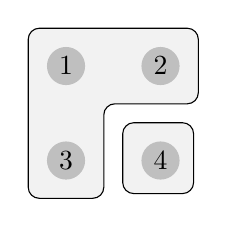
\begin{tikzpicture}[>=latex,scale=.6]
    
    % Possibilities    
    \draw[opaque,rounded corners]     
    (-1.8,0) -- (-1.8,1.8) -- (1.8, 1.8) -- (1.8,.2)
    -- (-.2, .2)
    -- (-.2,-1.8) -- (-1.8,-1.8) -- (-1.8,0);
    \draw[opaque,rounded corners] (.2,-.2) rectangle (1.7, -1.7);
    
    % Indices
    \draw (-1,1) node[index gray] (yy) {$1$};
    \draw (1,1) node[index gray] (yn) {$2$};
    \draw (-1,-1) node[index gray] (ny) {$3$};
    \draw (1,-1) node[index gray] (nn) {$4$};
  	
  	\end{tikzpicture}
    \caption{The model $M$ with the proposition $[?!(Ra \lor Rb)]$.}
    \label{fig:Example Model}
\end{figure}

\noindent In Section \ref{sec:Models} we have seen how we can represent this model in Haskell, i.e. $M$ corresponds to \verb|myModel|. Similarly, we have already seen the implementation of $?!(Ra \lor Rb)$ as \verb|myForm|. Lastly, we can compute the alternatives of the proposition $[?!(Ra \lor Rb)$ in GHCI as follows:
\begin{showCode}
*InqBSemantics> alt myModel myForm
\end{showCode}
\noindent This will return the following list of lists, which corresponds exactly to the alternatives in the figure.
\begin{showCode}
[[1,2,3],[4]]
\end{showCode}

\input{lib/ModelChecker.lhs}

\input{lib/HelperFunctions.lhs}

\input{test/Tests.lhs}

\section{Conclusion}\label{sec:Conclusion}
% \begin{itemize}
%     \item Samenvatting van wat we gedaan hebben
%     \item Shortcomings:
%         \begin{itemize}
%             \item Geen relatiesymbolen, maar relaties direct.
%             \item Geen implementatie van quantifiers in arbitrary instance
%         \end{itemize}
%     \item Uitbreidingen:
%         \begin{itemize}
%             \item Shortcomings verhelpen
%             \item Uitbreiden naar IEL
%             \item Implementeren voor \textit{InqI}.
%         \end{itemize}
% \end{itemize}

In this report we gave a concise introduction to the most basic framework of inquisitive semantics (\textsf{InqB}). We then implemented the models, syntax and semantics of \textsf{InqB} in Haskell. Thereafter, we combined these to create a model checker. Lastly, we used QuickCheck to check several facts about the framework \textsf{InqB}. Thereby we have created a tool that can be used to evaluate more complex models and formulas, and to check complex facts about \textsf{InqB}.

However, our implementation of \textsf{InqB} has two shortcomings. Firstly, as discussed in Section \ref{sec:Models}, we have omitted an interpretation function. This allowed us to give a simpler, more explicit manner of defining an arbitrary model. However, the downside of this is that formulas do not contain relation symbols but actual relations. Consequently, we can only define a formula relative to a model, making it impossible to evaluate the same formula in several different models.

Secondly, our \verb|Arbitrary| instance does not allow for arbitrary formulas containing quantifiers. This does not make our system less expressive, as quantifiers can be expressed using conjunction and disjunction in finite models. However, it would be an improvement to allow for the more succinct representation of formulas using quantifiers.

Our implementation can be improved by overcoming these two shortcomings. In sections \ref{sec:Models} and \ref{sec:InqBSyntax} we have discussed possible approaches for these improvements. Our model checker could also be extended to implement Inquisitive Epistemic Logic (\textsf{IEL}) which is a proper extension of \textsf{InqB}. Furthermore, an implementation for inquisitive semantics using intuitionistic logic rather than classical logic (\textsf{InqI}), would be an interesting subject for future research.



\addcontentsline{toc}{section}{Bibliography}
\bibliographystyle{alpha}
\bibliography{references.bib}

\end{document}
